% Options for packages loaded elsewhere
\PassOptionsToPackage{unicode}{hyperref}
\PassOptionsToPackage{hyphens}{url}
%
\documentclass[
  11pt,
]{article}
\usepackage{amsmath,amssymb}
\usepackage{iftex}
\ifPDFTeX
  \usepackage[T1]{fontenc}
  \usepackage[utf8]{inputenc}
  \usepackage{textcomp} % provide euro and other symbols
\else % if luatex or xetex
  \usepackage{unicode-math} % this also loads fontspec
  \defaultfontfeatures{Scale=MatchLowercase}
  \defaultfontfeatures[\rmfamily]{Ligatures=TeX,Scale=1}
\fi
\usepackage{lmodern}
\ifPDFTeX\else
  % xetex/luatex font selection
\fi
% Use upquote if available, for straight quotes in verbatim environments
\IfFileExists{upquote.sty}{\usepackage{upquote}}{}
\IfFileExists{microtype.sty}{% use microtype if available
  \usepackage[]{microtype}
  \UseMicrotypeSet[protrusion]{basicmath} % disable protrusion for tt fonts
}{}
\makeatletter
\@ifundefined{KOMAClassName}{% if non-KOMA class
  \IfFileExists{parskip.sty}{%
    \usepackage{parskip}
  }{% else
    \setlength{\parindent}{0pt}
    \setlength{\parskip}{6pt plus 2pt minus 1pt}}
}{% if KOMA class
  \KOMAoptions{parskip=half}}
\makeatother
\usepackage{xcolor}
\usepackage[left=3cm,right=3cm,top=3cm,bottom=3cm]{geometry}
\usepackage{longtable,booktabs,array}
\usepackage{calc} % for calculating minipage widths
% Correct order of tables after \paragraph or \subparagraph
\usepackage{etoolbox}
\makeatletter
\patchcmd\longtable{\par}{\if@noskipsec\mbox{}\fi\par}{}{}
\makeatother
% Allow footnotes in longtable head/foot
\IfFileExists{footnotehyper.sty}{\usepackage{footnotehyper}}{\usepackage{footnote}}
\makesavenoteenv{longtable}
\usepackage{graphicx}
\makeatletter
\newsavebox\pandoc@box
\newcommand*\pandocbounded[1]{% scales image to fit in text height/width
  \sbox\pandoc@box{#1}%
  \Gscale@div\@tempa{\textheight}{\dimexpr\ht\pandoc@box+\dp\pandoc@box\relax}%
  \Gscale@div\@tempb{\linewidth}{\wd\pandoc@box}%
  \ifdim\@tempb\p@<\@tempa\p@\let\@tempa\@tempb\fi% select the smaller of both
  \ifdim\@tempa\p@<\p@\scalebox{\@tempa}{\usebox\pandoc@box}%
  \else\usebox{\pandoc@box}%
  \fi%
}
% Set default figure placement to htbp
\def\fps@figure{htbp}
\makeatother
\setlength{\emergencystretch}{3em} % prevent overfull lines
\providecommand{\tightlist}{%
  \setlength{\itemsep}{0pt}\setlength{\parskip}{0pt}}
\setcounter{secnumdepth}{-\maxdimen} % remove section numbering
\ifLuaTeX
\usepackage[bidi=basic]{babel}
\else
\usepackage[bidi=default]{babel}
\fi
\babelprovide[main,import]{spanish}
% get rid of language-specific shorthands (see #6817):
\let\LanguageShortHands\languageshorthands
\def\languageshorthands#1{}
\usepackage{caption}
\captionsetup[table]{position=bottom,labelformat=default,labelsep=colon,name=Tabla}
\captionsetup[figure]{labelformat=default,labelsep=colon,name=Figura}
\usepackage{booktabs}
\usepackage{longtable}
\usepackage{array}
\usepackage{multirow}
\usepackage{wrapfig}
\usepackage{float}
\usepackage{colortbl}
\usepackage{pdflscape}
\usepackage{tabu}
\usepackage{threeparttable}
\usepackage{threeparttablex}
\usepackage[normalem]{ulem}
\usepackage{makecell}
\usepackage{xcolor}
\usepackage{bookmark}
\IfFileExists{xurl.sty}{\usepackage{xurl}}{} % add URL line breaks if available
\urlstyle{same}
\hypersetup{
  pdflang={es-ES},
  hidelinks,
  pdfcreator={LaTeX via pandoc}}

\author{}
\date{\vspace{-2.5em}}

\begin{document}

\begin{titlepage}
    \centering
    \makebox[\textwidth]{
    
\includegraphics[width=0.7\textwidth]{logo_facultad.png}
    } \par 
    \vspace{3cm}
    {\scshape\Huge Trabajo Práctico Estadistica No Parametrica \par}
    \vspace{3cm}
    \vfill
    {\Large Integrantes: \par}
    {\Large Coveñas Zavaleta Cristian Nahuel\\
            Cañizares María Inés\\
            Roura Agustina \par}
    \vfill
    {\large Octubre 2025 \par}
\end{titlepage}

\section{Introducción}\label{introducciuxf3n}

La fibrosis hepática es un proceso en el que el hígado produce y acumula
en exceso una sustancia llamada matriz extracelular, compuesta
principalmente por colágeno. Este exceso genera una especie de
``cicatriz interna'' que altera el funcionamiento normal del órgano. Con
el tiempo, la acumulación de colágeno y el ambiente inflamatorio que se
forma pueden favorecer la aparición del carcinoma hepatocelular (HCC),
la forma más común de cáncer de hígado. Las células estelares hepáticas
(HSC) son las principales responsables de este proceso: cuando el hígado
sufre algún daño, estas células se activan y comienzan a producir
grandes cantidades de colágeno. Por ello, encontrar maneras de evitar o
reducir esta activación es clave para prevenir o tratar la enfermedad
hepática avanzada y el HCC.

En este trabajo se buscó evaluar el potencial antifibrogénico de una
combinación de dos compuestos, Metformina y Ácido Lipoico, en células
estelares hepáticas cultivadas en laboratorio. El objetivo fue
determinar bajo qué condiciones experimentales (control, activación con
suero fetal al 10\% o activación con los compuestos) se produce una
mayor o menor cantidad de colágeno en la superficie de las células, lo
que refleja directamente su nivel de actividad fibrogénica.

Para ello, se trabajó con cuatro grupos de muestras independientes de
células, cada uno sometido a un tipo distinto de medio de cultivo. La
variable de interés mide la proporción de la superficie celular ocupada
por gránulos de colágeno, lo que permite comparar de forma cuantitativa
la respuesta entre grupos.

\section{Analisis descriptivo}\label{analisis-descriptivo}

En primer lugar, se procedió a realizar un análisis descriptivo de la
variable Superficie de Colágeno sobre Superficie Celular (SColSCel)
mediante el uso de una tabla descriptiva y un diagrama de caja (Figura
1), el cual mostró diferencias marcadas entre los tratamientos
evaluados.

\begin{longtable}[t]{ccccccccc}
\caption{\label{tab:unnamed-chunk-3}Resumen descriptivo de Superficie de Colágeno Sobre Superficie Celular por tratamiento}\\
\toprule
Tratamiento & N & Media & Mediana & Desvío Estándar & Minimo & Cuartil 1 & Cuartil 2 & Máximo\\
\midrule
SFB 1\% & 29 & 0.116 & 0.098 & 0.078 & 0.012 & 0.047 & 0.171 & 0.295\\
SFB 10\% & 17 & 0.224 & 0.215 & 0.086 & 0.115 & 0.171 & 0.259 & 0.448\\
SFB1\%+MA & 11 & 0.071 & 0.066 & 0.036 & 0.017 & 0.048 & 0.090 & 0.142\\
SFB10\%+MA & 28 & 0.051 & 0.048 & 0.017 & 0.025 & 0.041 & 0.058 & 0.099\\
\bottomrule
\end{longtable}

El tratamiento SFB 10\% presentó los valores medios y medianos más
elevados (0.22), acompañado de la mayor variabilidad, lo que podría
indicar una mayor formación de colágeno y mayor variabilidad entre las
mediciones. Los tratamientos SFB1\%+MA y SFB10\%+MA mostraron los
valores más bajos de colágeno (0.071 y 0.051, respectivamente) y menor
variabilidad, sugiriendo un efecto inhibidor sobre la formación de
colágeno al incorporar metformina y/o ácido lipoico. El tratamiento SFB
1\% (considerado como grupo control) presentó valores intermedios (media
= 0.116, mediana = 0.098), inferiores a SFB 10\% pero superiores a los
tratamientos combinados.

\begin{figure}

{\centering 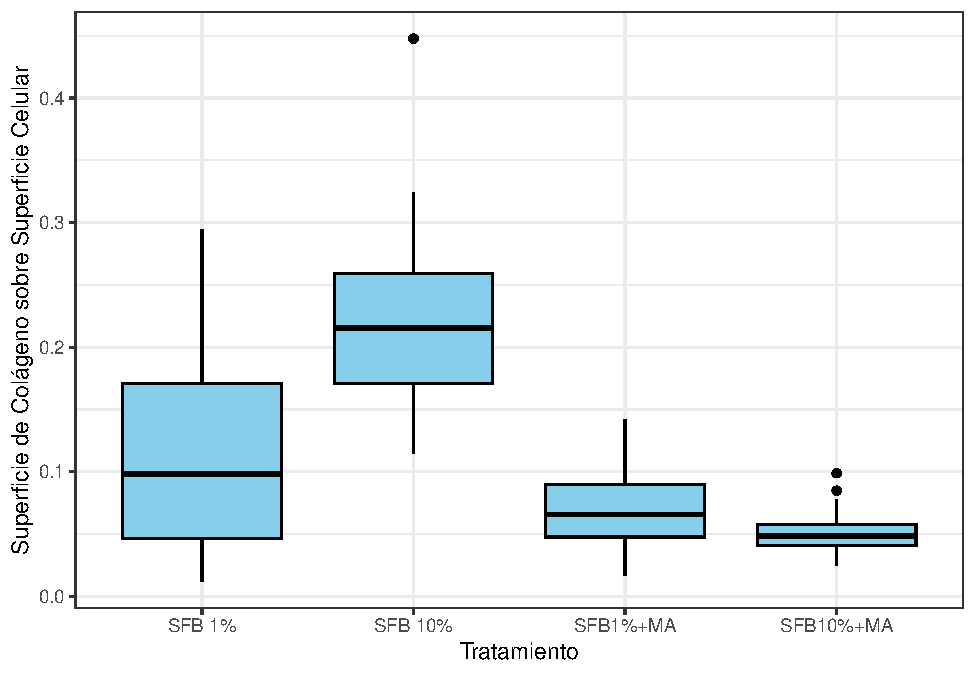
\includegraphics[width=0.55\linewidth,height=0.35\textheight]{Trabajo-Practico-NP_files/figure-latex/unnamed-chunk-4-1} 

}

\caption{Distribución de Superficie de Colágeno sobre Superficie Celular por tratamiento}\label{fig:unnamed-chunk-4}
\end{figure}

Además, en la Figura 1 se observaron algunos valores atípicos en todos
los grupos, aunque la tendencia general indicó que la presencia de
Metformina y Ácido lipoico disminuye la proporción de colágeno en la
superficie de las células.

Los resultados sugieren que la combinación de SFB con metformina y ácido
lipoico (+MA) reduce de manera consistente la superficie de colágeno
sobre las células.

\begin{figure}

{\centering 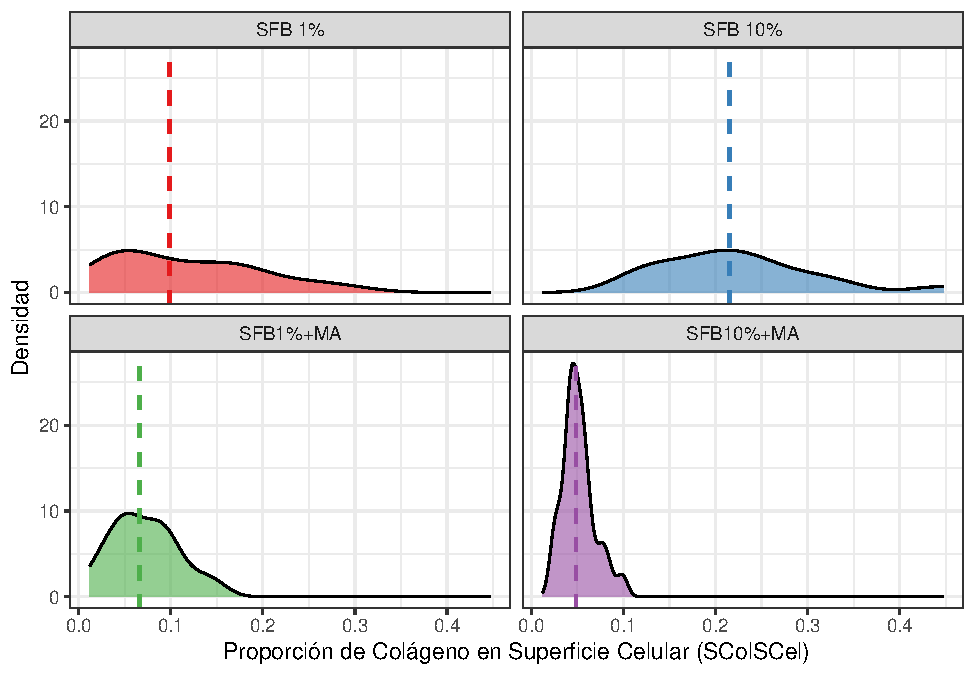
\includegraphics[width=0.55\linewidth,height=0.35\textheight]{Trabajo-Practico-NP_files/figure-latex/unnamed-chunk-5-1} 

}

\caption{Distribución de la Proporción de Colágeno por Tratamiento}\label{fig:unnamed-chunk-5}
\end{figure}
\newpage

La Figura 2 sugiere que la forma de las distribuciones para cada
tratamiento muestra un alejamiento de la normalidad, con asimetrías
visibles y posibles acumulaciones de valores en los extremos. Por esta
razón y el hecho de que la variable en análisis es una proporción,se
resalta que la aplicación de un test de normalidad no es apropiada.

\section{Análisis estadístico}\label{anuxe1lisis-estaduxedstico}

Luego del análisis descriptivo, que permitió observar tendencias
generales y posibles diferencias entre los tratamientos, se continuó con
un análisis estadístico para comprobar si esas diferencias son
significativas. Antes de ello, se evaluó si los datos cumplían las
condiciones necesarias para aplicar pruebas tradicionales basadas en la
normalidad.

Se evaluó si las observaciones siguen una distribución normal, para ello
se aplicó la prueba de Lilliefors de manera independiente a cada grupo
de tratamiento. Esta prueba compara la distribución empírica acumulada
de los datos con la función de distribución normal.

\begin{longtable}[]{@{}lc@{}}
\caption{Prueba de Normalidad de Lilliefors por Grupo de
Tratamiento}\tabularnewline
\toprule\noalign{}
Tratamiento & P-Value \\
\midrule\noalign{}
\endfirsthead
\toprule\noalign{}
Tratamiento & P-Value \\
\midrule\noalign{}
\endhead
\bottomrule\noalign{}
\endlastfoot
SFB 1\% & 0.1363 \\
SFB 10\% & 0.4464 \\
SFB1\%+MA & 0.9207 \\
SFB10\%+MA & 0.2976 \\
\end{longtable}

Los resultados mostraron valores de p superiores a 0.05 en todos los
tratamientos. Por lo tanto, se concluye con un nivel de significación
del 5\% que no hay evidencia muestral suficiente para decir que la
Superficie de Colágeno sobre Superficie Celular (SColSCel) no sigue una
distribución normal en cada tratamiento.

Asimismo, se analizó la homogeneidad de varianzas (homocedasticidad)
mediante la prueba de Levene. Los resultados indicaron que este supuesto
no se cumplía, desaconsejando el uso de métodos paramétricos
tradicionales.

\begin{longtable}[]{@{}cccc@{}}
\caption{Resultados de la Prueba de Levene}\tabularnewline
\toprule\noalign{}
Estadístico F & gl1 & gl2 & P-Value \\
\midrule\noalign{}
\endfirsthead
\toprule\noalign{}
Estadístico F & gl1 & gl2 & P-Value \\
\midrule\noalign{}
\endhead
\bottomrule\noalign{}
\endlastfoot
10.6844 & 3 & 81 & 0 \\
\end{longtable}

Como se puede observar, este supuesto no se cumplió, lo cual no se
sustenta la opción de continuar el análisis implementando métodos de
análisis paramétricos.

Además, dado que la variable respuesta se expresa como proporción y que
los gráficos de densidad muestran distribuciones asimétricas, no resulta
adecuado asumir normalidad ni homocedasticidad. Por esta razón, se optó
por métodos estadísticos no paramétricos, que permiten comparar los
tratamientos sin depender de estos supuestos.

\emph{Condiciones que generan mayor y menor producción de colágeno en
promedio}

Se decidió aplicar la prueba de Kruskal--Wallis para evaluar diferencias
entre los grupos, complementada con pruebas de comparaciones múltiples
que permitieron identificar los tratamientos con diferencias
significativas. Estos procedimientos brindan una evaluación más precisa
de la eficacia potencial de la combinación de Metformina y Ácido Lipoico
como estrategia antifibrogénica.

Se formuló como hipótesis principal que la proporción de colágeno
mediano es la misma entre los cuatro tratamientos aplicados a las
Células Estelares Hepáticas (HSC), esperando que alguna condición de
activación fibrogénica presentara una mediana diferente a las demás.

\begin{longtable}[]{@{}ccc@{}}
\caption{Resultados de la Prueba de Kruskal-Wallis para SColSCel por
Tratamiento}\tabularnewline
\toprule\noalign{}
Estadística & G.L. (Grados de Libertad) & P-Value \\
\midrule\noalign{}
\endfirsthead
\toprule\noalign{}
Estadística & G.L. (Grados de Libertad) & P-Value \\
\midrule\noalign{}
\endhead
\bottomrule\noalign{}
\endlastfoot
37.936 & 3 & 0 \\
\end{longtable}

Los resultados del test de Kruskal--Wallis indicaron una diferencia
significativa entre los grupos (\(H = 37.936\), \(p < 0.0001\)). Esto
permite rechazar la hipótesis nula de igualdad de medianas y confirma
que las condiciones de cultivo y la inclusión de los compuestos
antifibrogénicos modifican de manera significativa la tendencia central
de la actividad fibrogénica de las HSC.

Para identificar qué tratamientos se diferenciaban específicamente del
control, se realizaron comparaciones múltiples mediante la prueba de
Dunn con ajuste de Holm. El objetivo fue determinar cuáles condiciones
generaban mayor o menor producción de colágeno en promedio.

\begin{longtable}[]{@{}cc@{}}
\caption{Comparaciones por Pares (Dunn-Holm) con el Grupo Control (SFB
1\%)}\tabularnewline
\toprule\noalign{}
Comparación & P-Value \\
\midrule\noalign{}
\endfirsthead
\toprule\noalign{}
Comparación & P-Value \\
\midrule\noalign{}
\endhead
\bottomrule\noalign{}
\endlastfoot
SFB 1\% vs SFB 10\% & 0.0010 \\
SFB 1\% vs SFB1\%+MA & 0.1344 \\
SFB 1\% vs SFB10\%+M & 0.0039 \\
\end{longtable}

Los resultados mostraron diferencias estadísticamente significativas
entre el control (SFB 1\%) y los tratamientos SFB 10\% y SFB 10\%+MA
(\(p < 0.05\)), mientras que no se detectaron diferencias significativas
con el tratamiento SFB 1\%+MA. Estos hallazgos sugieren que las
condiciones asociadas a concentraciones más altas de SFB, especialmente
combinadas con Metformina y Ácido Lipoico, inducen un aumento en la
proporción de colágeno en superficie celular en comparación con el
control, mientras que la combinación con SFB 1\%+MA no genera cambios
significativos.

\emph{Condiciones que generan mayor o menor variabilidad en producción
de colágeno}

Con el fin de identificar las condiciones que generan mayor o menor
variabilidad en la producción de colágeno, se evaluó la dispersión de la
proporción de colágeno en superficie celular (SColSCel) entre los
tratamientos. Dado que la variable respuesta es una proporción y no se
cumple el supuesto de normalidad, se aplicó la prueba de Levene robusta
basada en la mediana (Brown--Forsythe), la cual permite contrastar
diferencias en la variabilidad de manera no paramétrica.

\begin{longtable}[]{@{}cccc@{}}
\caption{Resultados de la Prueba de Levene}\tabularnewline
\toprule\noalign{}
Estadístico F & gl1 & gl2 & P-Value \\
\midrule\noalign{}
\endfirsthead
\toprule\noalign{}
Estadístico F & gl1 & gl2 & P-Value \\
\midrule\noalign{}
\endhead
\bottomrule\noalign{}
\endlastfoot
10.6844 & 3 & 81 & 0 \\
\end{longtable}

Los resultados de la prueba indicaron que existían diferencias
significativas en la dispersión entre los grupos (𝑝 \textless{} 0.0001),
lo que sugiere que existe evidencia muestral suficiente para afirmar que
la variabilidad de la producción de colágeno sobre la superficie celular
(SColSCel) difiere en al menos uno de los cuatro tratamientos. Esta
prueba permite identificar cuáles condiciones generan una producción de
colágeno más consistente y cuáles presentan mayor dispersión.

El análisis descriptivo mostró que SFB10\%+MA presentó la menor
variabilidad, indicando una producción de colágeno más consistente,
mientras que SFB 10\% mostró la mayor dispersión, reflejando mayor
heterogeneidad en la respuesta de las células.

\newpage

\section{Conclusión}\label{conclusiuxf3n}

El análisis permitió evaluar el posible efecto antifibrogénico de la
combinación de Metformina y Ácido Lipoico (MA) en Células Estelares
Hepáticas (HSC), considerando como variable principal la proporción de
Colágeno sobre la Superficie Celular (SColSCel). Dado que esta variable
representa una proporción y mostró distribuciones asimétricas en los
diagramas de densidad (Figura 2), se decidió aplicar métodos
estadísticos no paramétricos, que no dependen del supuesto de
normalidad. Esta decisión asegura que las conclusiones sean más
confiables, incluso si los datos no siguen una distribución normal, a
pesar de que la prueba de Lilliefors no detectó desviaciones
significativas de normalidad (Tabla 2).

Los resultados descriptivos ya mostraron diferencias claras entre los
tratamientos. El grupo sometido al tratamiento de activación fibrogénica
(SFB 10\%) presentó la mediana más alta (0.215), mientras que el
tratamiento combinado SFB 10\%+MA tuvo la mediana más baja (0.048) y la
menor variabilidad (Tabla 1).

El análisis inferencial comenzó con la prueba de Kruskal-Wallis, que
confirmó la existencia de diferencias significativas entre los
tratamientos (\(H = 37.936, p < 0.0001\)). Esto permitió concluir que
las medianas de SColSCel no eran iguales entre los grupos y avanzar
hacia comparaciones más específicas.

Posteriormente, se aplicó la prueba de Dunn con ajuste de Holm para
comparar cada tratamiento con el grupo control (SFB 1\%). Los resultados
mostraron que el tratamiento SFB 10\% fue significativamente diferente
del control (\(p = 0.0010\)), validando el modelo experimental. De forma
aún más relevante, el grupo SFB 10\%+MA también fue significativamente
diferente (\(p = 0.0039\)), lo que indica que la combinación de
Metformina y Ácido Lipoico tiene un efecto inhibidor sobre la producción
de colágeno, llegando incluso a niveles inferiores a los observados en
el control. La única comparación sin diferencias significativas fue la
del grupo SFB 1\%+MA, lo que sugiere que el efecto protector se
manifiesta principalmente bajo condiciones de alta activación
fibrogénica.

Finalmente, la prueba de Levene (basada en la mediana) mostró
diferencias significativas en la variabilidad entre los grupos
(\(F = 10.6844, p < 0.0001\)). En conjunto con los resultados
descriptivos, esto indica que el tratamiento SFB 10\%+MA no solo redujo
la cantidad de colágeno, sino que también generó una respuesta celular
más homogénea y estable.

En síntesis, los resultados obtenidos confirman de manera clara la
hipótesis principal del estudio: la combinación de Metformina y Ácido
Lipoico (MA) presenta un alto potencial antifibrogénico en las Células
Estelares Hepáticas.

Incluso bajo condiciones diseñadas para inducir una fuerte producción de
colágeno (SFB 10\%), la presencia de los compuestos Metformina y Acido
Lipoico logró reducir notablemente su acumulación. En el grupo SFB
10\%+MA, la cantidad de colágeno fue menor no solo que en las células
activadas, sino también que en el grupo control (SFB 1\%). Este hallazgo
demuestra que el tratamiento puede no solo detener el daño, sino también
revertir parcialmente la activación celular. Además, la baja
variabilidad observada en este grupo sugiere que el efecto reductor de
Metformina y Ácido Lipóico es consistente y predecible, lo cual es una
característica deseable para cualquier enfoque terapéutico.

En conclusión, la combinación de Metformina y Ácido Lipóico surge como
una estrategia prometedora para el tratamiento de la fibrosis hepática,
ya que combina una fuerte reducción en la producción de colágeno con una
respuesta celular estable. Estos resultados experimentales respaldan la
necesidad de continuar con estudios adicionales que evalúen su seguridad
y eficacia, abriendo la posibilidad de nuevas alternativas para prevenir
o tratar la enfermedad hepática avanzada y el carcinoma hepatocelular
(HCC).

\section{Anexo}\label{anexo}

\subsection{1 Prueba de Normalidad para las muestras - Test de bondad de
ajuste de
Lilliefors}\label{prueba-de-normalidad-para-las-muestras---test-de-bondad-de-ajuste-de-lilliefors}

\begin{itemize}
\item
  Hipótesis:
  \[H_0) \ X_i \sim Normal \ \ \text{vs} \ \ H_1) \ X_i \nsim Normal\]
  Con \(X_i\): muestra aleatoria del tratamiento \(i\)-esimo.
  \(i = 1,4\) En particular se realizaron 4 test de normalidad para los
  distintos tratamientos.
\item
  Estadística: \(L_n = máx_x |S_n(X_i) - F_o(X_i)|\), mide la maxima
  diferencia entre la función de distribución acumulada empirica contra
  la funcion de distribución normal.
\item
  Regla de decisión:
  \(\text{Rechazo } H_0 \text{ si} \ L \ge L_{1 - \alpha}\)
\end{itemize}

\subsection{2 Condiciones de mayor y menor producción en promedio - Test
de
Kruskal--Wallis}\label{condiciones-de-mayor-y-menor-producciuxf3n-en-promedio---test-de-kruskalwallis}

\begin{itemize}
\item
  Hipótesis:
\item
  Estadística:
\item
  Regla de decisión:
\end{itemize}

\end{document}
